% !TEX root = ../main.tex
\chapter{Planning}
\label{Planning}
Following a number of supervisor meetings with Dr Pitt, a number of work items have been identified. A Gantt Chart was created to facilitate the planning and tracking of the project progress. A copy of the current Gantt Chart can be seen in Figure \ref{fig:GanttChart}. The Gantt Chart was a continuous working document which will be update as the project progresses. Tasks were added as new ideas for the project became available. 

\begin{figure}[h!]
\centering
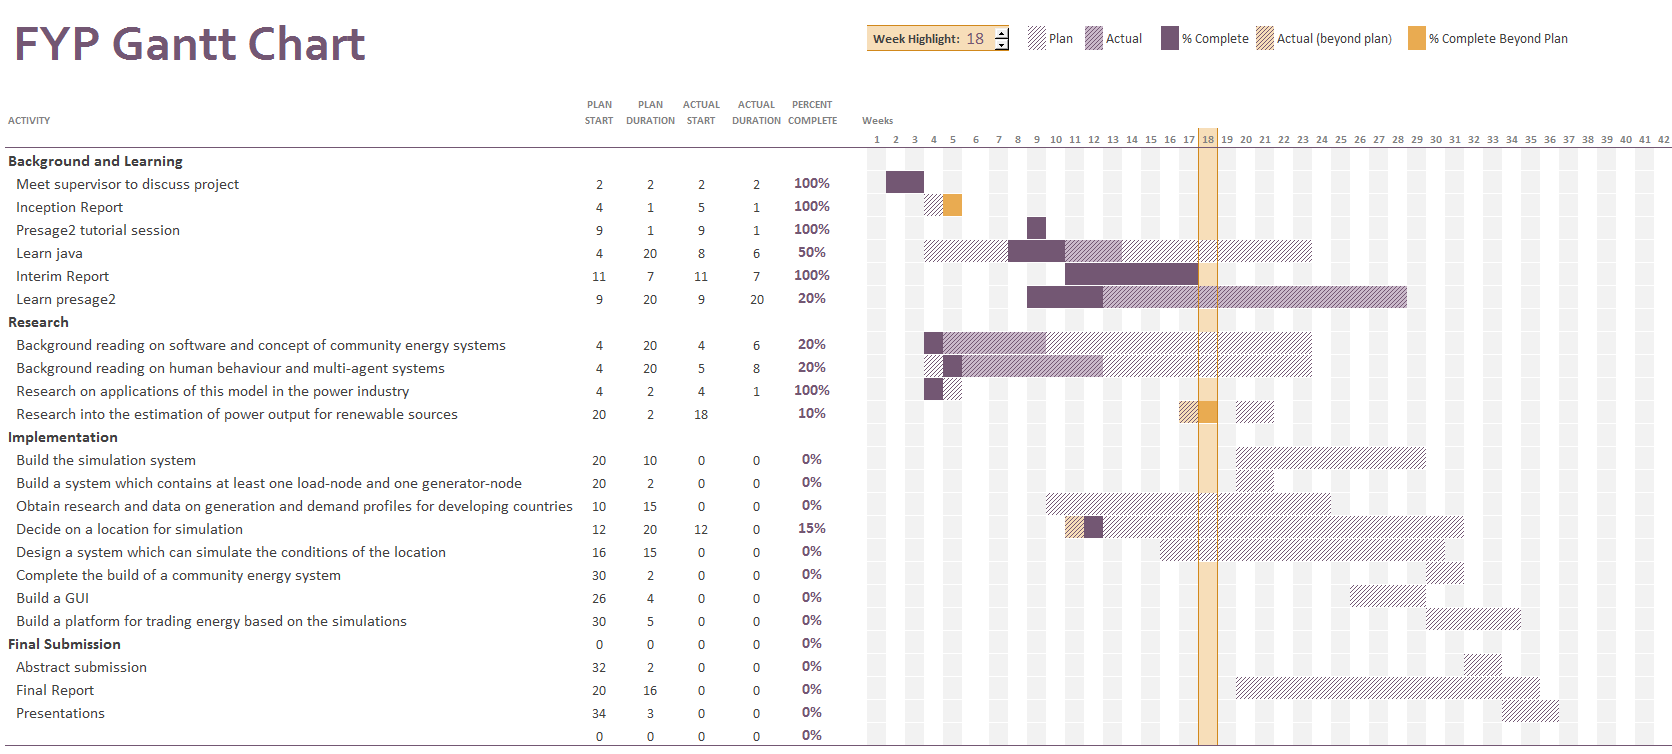
\includegraphics[scale=0.5, angle=90]{Images/GanttChart.png}
\caption{Up to date Gantt chart}
\label{fig:GanttChart}
\end{figure}

Throughout the year, the Gantt Chart was updated to reflect changing priorities, targets and difficulties as the projects progressed. The final project Gantt Chart can be seen below:
\pdfmarkupcomment[markup=Highlight,color=yellow]{ [[[[ "Include Gantt Chart here" ]]]]}{Highlight}
%Include Gantt Chart here